\section{Crystals}

\paragraph{Crystals}
Solid state physics, as we will study it, is concerned with crystals. A crystal is an arrangement of atoms which is repeated periodically. When developing the physics of crystals, we will assume their repetition to be infinite.

\paragraph{Basis}
The arrangement of atoms which is repeated in a crystal is termed the basis. Note the ambiguity in the choice of basis.

\paragraph{Lattices}
The set of points to which the basis is attached is termed the lattice. The ambiguities in the choices of basis and lattice are connected.

\paragraph{Bravais Lattices}
A Bravais lattice is a lattice such that the arrangement of lattice points looks exactly equal from any lattice point. This turns out to be equivalent to the lattice being infinite and symmetric under certain discrete translations. We will treat crystal lattices as Bravais lattices.

The two-dimensional Bravais lattices are the rectangular, square, hexagonal, centered rectangular and monoclinic lattices. Some are shown in figure \ref{fig:bravais2D}.

%TODO: Add the rest
\begin{figure}[!ht]
	\centering
	\subfloat[Square.]
	{
		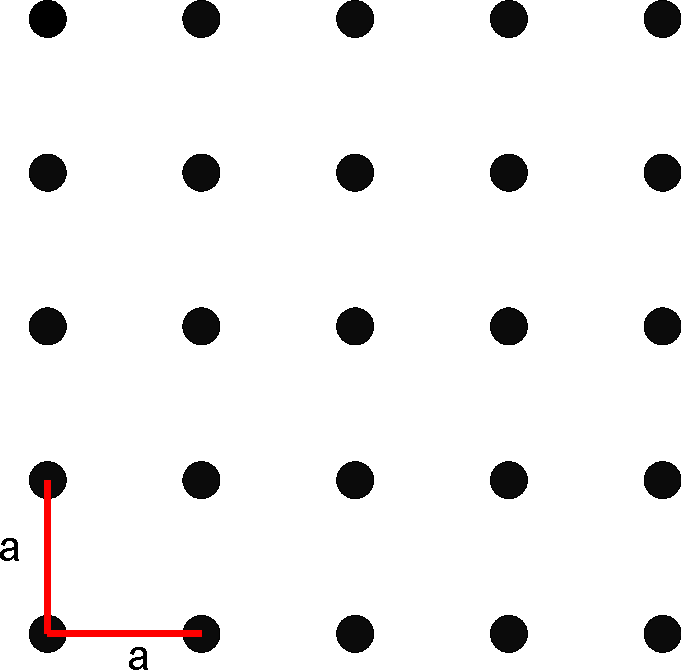
\includegraphics[width = 0.3\textwidth]{./Images/2d_square.pdf}
	}
	\hfil
	\subfloat[Rectangular.]
	{
		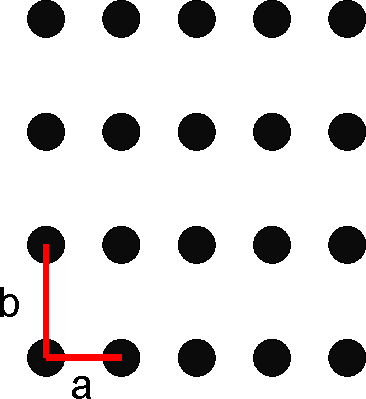
\includegraphics[width = 0.3\textwidth]{./Images/2d_rectangular.pdf}
	}
	\caption{Some Bravais lattices in two dimensions.}
	\label{fig:bravais2D}
\end{figure}

The three-dimensional lattices are more numerous, but can be divided into triclinic, monoclinic, orthorhombic, tetragonal, cubic, trigonal and hexagonal lattices.

%TODO: Add 3D Bravais lattices

\paragraph{Lattice Vectors}
The set $\{\vb{a}_{i}\}$ of lattice vectors of a Bravais lattice is the smallest possible set of vectors such that translating the lattice by $u_{i}\vb{a}_{i}$, where the $u_{i}$ are integers, leaves the lattice unchanged. For any given lattice, there are numerous ways to define the lattice vectors.

\paragraph{Primitive Lattice Vectors}
A set of lattice vectors is primitive if any two lattice points are connected by integer combinations of the lattice vectors.

\paragraph{Crystal Axes}
The crystal axes are a set of directions that span space. These may be chosen according to, for instance, the primitive lattice vectors or other directions connected to the symmetry of the lattice.

\paragraph{Crystal Cell}
The crystal cell is the repeat unit of the crystal. It may be constructed in an infinite number of ways.

\paragraph{Lattice Constants}
Lattice constants are a set of parameters defining the dimensions of the cell.

\paragraph{Primitive Cell}
The primitive cell is a minimum-volume cell. It contains only one lattice point, and is thus termed a unit cell.

\paragraph{Primitive Basis}
The primitive basis is the basis associated with the primitive cell.

\paragraph{Wigner-Seitz Cell}
The Wigner-Seitz Cell is the cell constructed by for any lattice point dividing space into two at the middle of and normal to the line between the point in question and all other points, and choosing the smallest region of space containing the point which is defined by the divisions of space.

\paragraph{Lattice Point Group}
The lattice point group is the group of operations which, applied about a lattice point (i.e. keeping this point fixed), leaves the lattice unchanged. Examples of possible fundamental operations include:
\begin{itemize}
	\item rotations.
	\item reflections.
\end{itemize}

\paragraph{Lattice Space Group}
The space group of the Bravais lattices is the group of symmetries of all Bravais lattices of a given dimensionality. It contains both point groups and translations.

\paragraph{$n$-Fold Rotations}
An $n$-fold rotation is a rotation operation such that it reduces to the identity operation when applied $n$ times. Lattices cannot be symmetric under $5$-fold rotation.

\paragraph{Crystal Planes}
In a cell it is useful to define crystallographic planes. These are indicated by a set of indices \cplane{hkl}, the computation of which we will return to. A bar above any element indicates that element to be negative.

A set of parallel planes such that all lattice points are contained in the set may be denoted \cpset{hkl}.

\paragraph{Crystallographic Directions}
Likewise we define crystallographic directions by the notation \cdir{uvw}. The indices are the set of the smallest integers such that they form a vector parallel to the one in question.

\paragraph{Random Stacking}
Randomly stacked crystals are formed by densely packed layers of atoms being stacked without long-range order in the stacking direction.

\paragraph{Polytopism}
Polytopism is a milder variation of random stacking, where the order of the stacked layers is extremely long-range.

%TODO: Add special structures

\paragraph{X-Ray Diffraction}
X-ray diffraction is the process of shining X-rays onto a material in order to characterize it. Before atomic physics, it was discovered that solids scattered X-rays intensely in specific directions, as opposed to light, which was reflected by the solid. In the context of solid-state physics, we can interpret this as crystal planes acting as diffraction grids that scatter the X-rays. This interpretation makes sense because the wavelength of X-rays is comparable to interatomic distances in a solid, consistent with the regime in which classical wave physics predicts that diffraction phenomena are significant, and the scattered light being localized is consistent with diffraction of other waves.

\paragraph{Bragg's Law}
Bragg's law was a first attempt at explaining X-ray diffraction patterns. To derive it, consider a solid composed of aligned and stacked atomic planes separated by a distance $d$ on which electromagnetic radiation of wavelength $\lambda$ is incident at angle $\theta$ to the planes, and suppose each plane reflects the radiation specularly (following the law of reflection) and elastically (preserving the wavelength). Comparing radiation reflected from two adjacent layers, the light in the lower layer travels a distance $2d\sin{\theta}$ longer. In order for the radiation from these layers to interfere constructively, we must have
\begin{align*}
	2d\sin{\theta} = n\lambda,\ n = 1, 2, \dots
\end{align*}
This is Bragg's law. It is a very rough description of X-ray diffraction, but predicts the phenomenology correctly. It also predicts that diffraction occurs for $\lambda < 2d$, which is why light, for instance, is not diffracted by solids.

\paragraph{Fourier Analysis and Reciprocal Space}
The translational symmetry of the lattice implies that the tools of Fourier analysis are applicable when studying solid-state physics. Any observable $A$ defined on the crystal lattice may be written as
\begin{align*}
	A = \sum\limits_{\vb{G}}A_{\vb{G}}e^{i\vb{G}\cdot\vb{r}}.
\end{align*}
The coefficients in the series expansion are given by
\begin{align*}
	A_{\vb{G}} = \frac{1}{V_{\text{cell}}}\integ[d]{\text{cell}}{}{\vb{r}}{A(\vb{r})e^{-i\vb{G}\cdot\vb{r}}}.
\end{align*}
In order for $A$ to be an observable, we must have $A_{-\vb{G}} = \cc{A_{\vb{G}}}$. The fact that $A$ is an observable on the crystal lattice implies that it must have the same symmetries - in particular translational symmetry. This implies
\begin{align*}
	A(\vb{r} + u_{i}\vb{a}_{i}) = A(\vb{r}) \implies u_{i}\vb{G}\cdot\vb{a}_{i} = 2\pi n
\end{align*}
where $n$ is an integer. This defines the set of allowed expansion coefficients in the Fourier expansion. The vectors $\vb{G}$ must have reciprocal length as their dimension, and thus belong to what is termed reciprocal space.

\paragraph{The Reciprocal Lattice}
The simplest choice of vectors satisfying
\begin{align*}
	u_{i}\vb{G}\cdot\vb{a}_{i} = 2\pi n
\end{align*}
is integer combinations of a set of vectors $\{\vb{b}_{i}\}$ such that $\vb{a}_{i}\cdot\vb{b}_{j} = 2\pi\delta_{ij}$. The set of vectors $\{\vb{b}_{i}\}$ thus defines a Bravais lattice in reciprocal space, termed the reciprocal lattice. In three dimensions, the explicit formula for the reciprocal lattice vectors is
\begin{align*}
	\vb{b}_{1} = \frac{2\pi}{V_{\text{cell}}}\vb{a}_{2}\times\vb{a}_{3},\ V_{\text{cell}} = \vb{a}_{1}\cdot(\vb{a}_{2}\times\vb{a}_{3})
\end{align*}
with cyclic permutation of the indices yielding the other two.

\paragraph{Crystal Planes and the Reciprocal Lattice}
Assume that there is a lattice point at the origin and that the closest crystal plane with orientation specified by the unit normal vector $\vb{n}$ is a distance $d$ from the origin. Any plane parallel to the plane in question is described by
\begin{align*}
	\vb{r}\cdot\vb{n} = md,\ m = 0, \pm 1, \dots
\end{align*}

Consider now a translation by $\vb{T}$ such that the lattice is left invariant. Assuming the translation to be between lattice points, the translation must satisfy the equation of some crystal plane, implying
\begin{align*}
	\vb{T}\cdot\vb{n} = md.
\end{align*}
In particular, if the translation is to a point in a plane adjacent to the origin, we have
\begin{align*}
	\vb{T}\cdot\frac{2\pi}{d}\vb{n} = 2\pi.
\end{align*}
Comparing this to the definition of the reciprocal lattice implies that the plane is normal to a reciprocal lattice vector
\begin{align*}
	\vb{G} = \frac{2\pi}{d}\vb{n}.
\end{align*}
This is the shortest reciprocal lattice vector describing the plane.

\paragraph{Miller Indices}
Returning to the indexing system for crystal planes, we may decompose the normal vector as
\begin{align*}
	\vb{G} = h\vb{b}_{1} + k\vb{b}_{2} + l\vb{b}_{3}.
\end{align*}
These indices are exactly the indices used to describe a crystal plane, and are termed Miller indices. As $\vb{G}$ is the shortest vector describing the plane, the indices cannot contain any common factors.

The Miller indices may also be computed from the real lattice according to the following rules:
\begin{enumerate}
	\item For each axis, defined by the lattice vectors, identify the intercepts of the plane with the axis as units of the lattice parameters.
	\item Compute the reciprocals of each intercept.
	\item Reduce to three integers with the same ratio.
\end{enumerate}

\paragraph{Interplanar Distances}
Using the final result describing the normal of a given set of crystal planes, we obtain
\begin{align*}
	d = \frac{2\pi}{\abs{\vb{G}_{hkl}}},
\end{align*}
which is true for any Bravais lattice.

\paragraph{Diffraction by Solids}
Using the language of Fourier analysis and reciprocal space, we will try to derive a more sophisticated diffraction condition.

To do this, consider a crystal exposed to far-field radiation described by a wave vector $\vb{k}$ which is scattered elastically by the crystal in an arbitrary direction and observed in the far-field region in some direction, in which the wave vector is $\vb{k}^{\prime}$. Considering the interference between two points displaced by $\vb{r}$, the phase difference between the radiation from the two points is $(\vb{k} - \vb{k}^{\prime})\cdot\vb{r}$. Supposing that the amplitude of the scattered wave is proportional to the electron density (or, really, any property defined on the lattice), the total scattered amplitude is proportional to the (confusingly termed) scattering amplitude
\begin{align*}
	F = \integ[d]{}{}{\vb{r}}{n(\vb{r})e^{i(\vb{k} - \vb{k}^{\prime})\cdot\vb{r}}}.
\end{align*}
Adding the series expansion of the electron density yields
\begin{align*}
	F = \integ[d]{}{}{\vb{r}}{\sum\limits_{\vb{G}}n_{\vb{G}}e^{i\vb{G}\cdot\vb{r}}e^{-i\Delta\vb{k}\cdot\vb{r}}} = \integ[d]{}{}{\vb{r}}{\sum\limits_{\vb{G}}n_{\vb{G}}e^{i(\vb{G} - \Delta\vb{k})\cdot\vb{r}}} = \sum\limits_{\vb{G}}\integ[d]{}{}{\vb{r}}{n_{\vb{G}}e^{i(\vb{G} - \Delta\vb{k})\cdot\vb{r}}}.
\end{align*}
For the case $\Delta\vb{k} = \vb{G}$ for any one particular reciprocal lattice vector, the exponential in this term vanishes, leaving a term $Vn_{\vb{G}}$. It can be shown that all other terms in the scattering amplitude vanish, yielding $F = Vn_{\vb{G}}$ for this case and $F = 0$ otherwise. The most fundamental diffraction condition is thus
\begin{align*}
	\Delta\vb{k} = \vb{G}.
\end{align*}

While we have in principle obtained a diffraction condition now, we can simplify it by using the fact that the scattering is inelastic. We obtain
\begin{align*}
	2\vb{k}\cdot\vb{G} + G^{2} = 0.
\end{align*}
It may be rewritten by swapping $\vb{G}$ for $-\vb{G}$, which is also a reciprocal lattice vector, to yield
\begin{align*}
	2\vb{k}\cdot\vb{G} = G^{2}.
\end{align*}

Note that this implies that information about the reciprocal lattice, and therefore the lattice itself, may be obtained from diffraction experiments.

\paragraph{Laue's Equations}
The fundamental diffraction criterion implies
\begin{align*}
	\Delta\vb{k}\cdot\vb{a}_{i} = 2\pi v_{i}
\end{align*}
for some integer $v_{i}$, simultaneously for all lattive vectors. This implies that reflections are only found at the intersection of three cones in reciprocal space. This is very strict, and such reflections must be found by sweeping in crystal orientation and/or wavelength or by chance.

\paragraph{The Ewald Sphere}
The Ewald sphere is a tool for visualizing the necessary conditions for diffractions. To construct it, draw the incident wave vector starting in a point such that it terminates in a reciprocal lattice point. From the starting point, draw a sphere of radius $k$. All reciprocal lattice points corresponding to a diffraction peak are found on this sphere.

\paragraph{Brillouin Zones}
To introduce the concept of Brillouin zones, rewrite the diffraction condition as
\begin{align*}
	\vb{k}\cdot\frac{1}{2}\vb{G} = \left(\frac{1}{2}G\right)^{2}.
\end{align*}
For a fixed $\vb{G}$, this equation defines the set of wave vectors terminating on the bisector of $\vb{G}$. This is similar to the construction of the Wigner-Seitz cell in real space, but now extended to construct zones using all points in the reciprocal lattice. Constructing these bisectors divides the reciprocal space into Brillouin zones (a single Brillouin zone is the combinations of all zones a fixed number of zones from the central zone). The central zone, which is the Wigner-Seitz cell in reciprocal space, is the first Brillouin zone.

\paragraph{Volume of the Brillouin Zone}
We would like to compute the volume of the Brillouin zone in terms of the volume of the unit cell. To do this, we note that the unit cell volume is given by
\begin{align*}
	V_{\text{c}} = \vb{a}_{1}\cdot(\vb{a}_{2}\times\vb{a}_{3}).
\end{align*}
Similarly, the volume of the Brillouin zone is given by
\begin{align*}
	V_{\text{r}} = \vb{b}_{1}\cdot(\vb{b}_{2}\times\vb{b}_{3}).
\end{align*}
The vector in the parenthesis is given by
\begin{align*}
	\vb{b}_{2}\times\vb{b}_{3} &= \frac{(2\pi)^{2}}{V_{\text{c}}^{2}}(\vb{a}_{3}\times\vb{a}_{1})\times (\vb{a}_{1}\times\vb{a}_{2}) \\
	                           &= \frac{(2\pi)^{2}}{V_{\text{c}}^{2}}((\vb{a}_{3}\cdot(\vb{a}_{1}\times\vb{a}_{2}))\vb{a}_{1} - (\vb{a}_{3}\cdot(\vb{a}_{1}\times\vb{a}_{1}))\vb{a}_{2}) \\
	                           &= \frac{(2\pi)^{2}}{V_{\text{c}}}\vb{a}_{1},
\end{align*}
and thus the volume of the Brillouin zone is given by
\begin{align*}
	V_{\text{r}} = \frac{(2\pi)^{3}}{V_{\text{c}}}.
\end{align*}

\paragraph{The Structure Factor and Atomic Form Factor}
The diffraction condition is stated in terms of reciprocal lattice vectors obtained from the primitive lattice vectors. However, especially in experimental contexts, the primitive unit cell is not the geometry of choice for studying materials. Instead, one can use inherent ambiguities in choices of repeat units of the crystal to study geometries with, for instance, more or simpler symmetries. When considering such geometries, the diffraction conditions is only necessary, not sufficient. We will now study diffraction for such cases.

Consider a crystal built up of some kind of cell, not necessarily a primitive one. When the diffraction condition is satisfied, i.e. $\Delta\vb{k} = \vb{G}$ for some reciprocal lattice vector corresponding to the chosen cell, the scattering amplitude for a crystal of $N$ cells becomes
\begin{align*}
	F = \integ[d]{}{}{\vb{r}}{n(\vb{r})e^{-i\vb{G}\cdot\vb{r}}} = N\integ[d]{\text{cell}}{}{\vb{r}}{n(\vb{r})e^{-i\vb{G}\cdot\vb{r}}} = NS_{\vb{G}},
\end{align*}
where we have introduced the structure factor $S_{\vb{G}}$, which describes the effect of the electron distribution in the cell on the scattering amplitude for a given diffraction peak.

Writing the electron density as a superposition of contributions from each atom in the basis (this decomposition is not unique, but somehow this is not a problem), we obtain
\begin{align*}
	S_{\vb{G}} = \integ[d]{\text{cell}}{}{\vb{r}}{\sum n_{j}(\vb{r} - \vb{r}_{j})e^{-i\vb{G}\cdot\vb{r}}}
\end{align*}
where the $\vb{r}_{j}$ are the positions of the atoms in the basis. We rewrite this as
\begin{align*}
	S_{\vb{G}} = \sum\integ[d]{\text{cell}}{}{\vb{r}}{n_{j}(\vb{r} - \vb{r}_{j})e^{-i\vb{G}\cdot\vb{r}}} = \sum e^{-i\vb{G}\cdot\vb{r}_{j}}\integ[d]{\text{cell}}{}{\vb{r}}{n_{j}(\vb{r})e^{-i\vb{G}\cdot\vb{r}}}.
\end{align*}
Defining the atomic form factor
\begin{align*}
	f_{j, \vb{G}} = \integ[d]{\text{cell}}{}{\vb{r}}{n_{j}(\vb{r})e^{-i\vb{G}\cdot\vb{r}}}
\end{align*}
we have
\begin{align*}
	S_{\vb{G}} = \sum f_{j, \vb{G}}e^{-i\vb{G}\cdot\vb{r}_{j}}.
\end{align*}
The requirement for diffraction is thus that $\Delta\vb{k} = \vb{G}$ and the structure factor being non-zero.

The atomic form factor of a single atom is closely connected to its valency. For instance, if the electron distribution is completely localized at the nucleus, we obtain
\begin{align*}
	f_{j, \vb{G}} = Z
\end{align*}
where $Z$ is the number of electrons in the atom. The relation to the number of electrons turns out to be true for the general case as well.

When observing electron distributions in solids, these appear close to those of free atoms. This does not mean that electrons are not distributed in a solid versus for free atoms, but that these corrections do not have a major effect on the atomic form factors. Thus it may be relevant to write these as
\begin{align*}
	f_{j, \vb{G}} = \integ[d]{}{}{\vb{r}}{n_{j}(\vb{r})e^{-i\vb{G}\cdot\vb{r}}}
\end{align*}
where the electron distribution is that of a free atom and the integration is performed over all of space.

The astute reader might have noticed that when considering the primitive unit cell of a crystal with one atom in the basis, the structure factor is trivial. However, this description is often chosen in these cases as well, and so one could ask whether this is necessary. The answer to the latter question is left to experimentalists, but I can confirm that this derivation neither adds nor subtracts to our knowledge for these cases. If you have chosen the primitive cell, the structure factor is trivial and diffraction occurs for every observation such that the diffraction criterion is satisfied. For other choices of cells, certain reciprocal lattice vectors will produce a structure factor equal to zero. This is because these do not correspond to reciprocal lattice vectors of the primitive cell. Someone should prove this more rigorously. Can we be sure that other choices of cells cover all possible reciprocal lattice vectors of the primitive cell? Yes, as non-primitive cells must have longer lattice vectors, corresponding to shorter reciprocal lattice vectors, implying that the reciprocal lattice vectors of the primitive cell should be possible to express as combinations of the reciprocal lattice vectors of the non-primitive cell.

\paragraph{Cohesive Energy}
The cohesive energy of a crystal is the energy required to separate the crystal into neutral free atoms at rest at infinite separation.

\paragraph{Types of Crystal Binding}
The different types of crystal binding and their origins are
\begin{itemize}
	\item van der Waals binding, which occurs due to fluctuating electric dipoles in atoms and molecules.
	\item ionic binding, which occurs due to Coulomb forces between ions.
	\item covalent binding, which occurs due to the filling of electron states localized between atoms.
	\item metal binding, where valence electrons form a gas throughout the crystal, the presence of which balances the repulsion between the metal atoms in the lattice.
\end{itemize}

\paragraph{van der Waals Energy}
%TODO: Derivation of van der Waals energy
The van der Waals interaction between two atoms in a crystal or molecule is modelled as a potential of the form
\begin{align*}
	V = 4\varepsilon\left(\left(\frac{\sigma}{R}\right)^{12} - \left(\frac{\sigma}{R}\right)^{6}\right)
\end{align*}
with a positive term from Pauli repulsion and a negative term from attraction between fluctuating dipoles.

For a crystal of $N$ atoms the cohesive energy due to van der Waals interaction becomes
\begin{align*}
	U = 2N\varepsilon\left(\sum\limits_{j}\left(\frac{\sigma}{R_{j}}\right)^{12} - \left(\frac{\sigma}{R_{j}}\right)^{6}\right).
\end{align*}
Re-expressing this in terms of nearest-neighbour distances $R$ in the lattice, we can write $R_{j} = p_{j}R$ to obtain
\begin{align*}
	U = 2N\varepsilon\left(\left(\frac{\sigma}{R}\right)^{12}\sum\limits_{j}\frac{1}{p_{j}^{12}} - \left(\frac{\sigma}{R}\right)^{6}\sum\limits_{j}\frac{1}{p_{j}^{6}}\right)
\end{align*}
where we have divided by two in order to distribute the interaction energy evenly between the atoms. The two summations are determined solely by the crystal structure.

\paragraph{Ionic Binding}
Ionic interactions between two atoms in a crystal are modelled as a potential of the form
\begin{align*}
	V = \lambda e^{-\frac{R_{ij}}{\rho}} \pm \frac{q^{2}}{4\pi\varepsilon_{0}R_{ij}}
\end{align*}
with a positive term from Pauli repulsion and a term from attraction between charged particles, the sign of which depending on the ions in question. The Pauli term is typically only included for nearest neighbours.

For a crystal of $N$ atoms the cohesive energy due to ionic interaction becoms
\begin{align*}
	U = N\left(Z\lambda e^{-\frac{R}{\rho}} + \sum\limits_{j}(-1)^{g(j)}\frac{q^{2}}{4\pi\varepsilon_{0}R_{ij}}\right)
\end{align*}
where we have introduced the function $g$ describing whether atom  $j$ has an equal or opposite charge to that of the atom in the origin. Re-expressing the Coulomb term in terms of nearest-neighbour distances we obtain
\begin{align*}
	U = N\left(Z\lambda e^{-\frac{R}{\rho}} - \alpha\frac{q^{2}}{4\pi\varepsilon_{0}R_{ij}}\right)
\end{align*}
where $Z$ is the coordination number of a given ion and
\begin{align*}
	\alpha = \sum\limits_{j}\frac{(-1)^{g(j)}}{p_{ij}}
\end{align*}
is termed the Madelung constant and depends only on the crystal structure.

\paragraph{Covalently Bound Solids}
Solids bound by covalent force have localized electrons due to the nature of the bonds in the solid, meaning that such bonds are typically found in insulators and semiconductors.

\paragraph{Metals}
Electrons in metals move around in a gas, hence metals are generally good conductors.

\paragraph{Atomic Radii}
The introduced parameters in the interaction potentials described above that have dimensions of length are essentially dependent on atomic radii. It turns out that atomic radii are largely independent of the composition of the material in which any given atom is found. However, they are significantly affected by coordination number.